\documentclass[9pt,xcolor=table]{beamer}
\usepackage[latin1]{inputenc}
\usepackage[english]{babel}
% \usepackage{graphics}
\usepackage{graphicx}
\usepackage{hyperref}
\usepackage{units}
\usepackage{amsmath}
\usepackage{amsfonts}
\usepackage{amssymb}
\usepackage{color, colortbl}
\usepackage{amsmath}
%\usepackage{wrapfig}
\usepackage[normalem]{ulem}
%\usepackage{multirow}
\usepackage{verbments}
\usepackage{textcomp}

\usetheme{MPICBG}

\def\cpp{\texttt{C++}}
\def\cpu{\texttt{CPU}}
\def\gpu{\texttt{GPGPU}}
\def\Cuda{\texttt{CUDA}}


\AtBeginSection[] 
{
\begin{frame}<beamer>
\frametitle{Outline}
\vspace{-1.5\baselineskip}
\begin{columns}[t]
  \begin{column}{.1\textwidth}
    \hfill
  \end{column}
  \begin{column}{.75\textwidth}
    \huge
    \tableofcontents[currentsection,hideallsubsections]
  \end{column}
  \begin{column}{.1\textwidth}
    \hfill
  \end{column}
\end{columns}
\end{frame}
}
   
\begin{document}
     
\pgfdeclareimage[height=1.5cm]{MPIlogo}{img/CBGlogo}
\titlegraphic{ \pgfuseimage{MPIlogo}  }
 
 
\title[PerfVsDesign]{Performance versus Design}
\subtitle{- Advanced Programming School 2014 -}
\author[P. Steinbach]{Peter Steinbach}
\date{}
\institute[MPI CBG]{Max Planck Institute of Molecular Cell Biology and Genetics\\Scientific Computing Facility}
\addtocounter{framenumber}{-1}
\renewcommand*\inserttotalframenumber{XX} 

 
{
\setbeamertemplate{footline}{} 
\maketitle
}

\begin{frame}[t]
\frametitle{Outline}
\vspace{-1.5\baselineskip}
\begin{columns}[t]
  \begin{column}{.1\textwidth}
    \hfill
  \end{column}
  \begin{column}{.75\textwidth}
    \huge
    \tableofcontents[hideallsubsections]
  \end{column}
  \begin{column}{.1\textwidth}
    \hfill
  \end{column}
\end{columns}
\end{frame}

\section*{Before we start ...}
\begin{frame}
\frametitle{\insertsection{}}
\begin{center}
  \huge\textcolor{red}{Warning!}
\end{center}
\begin{columns}[c]
  \begin{column}{.35\textwidth}
    \begin{figure}[htb]
      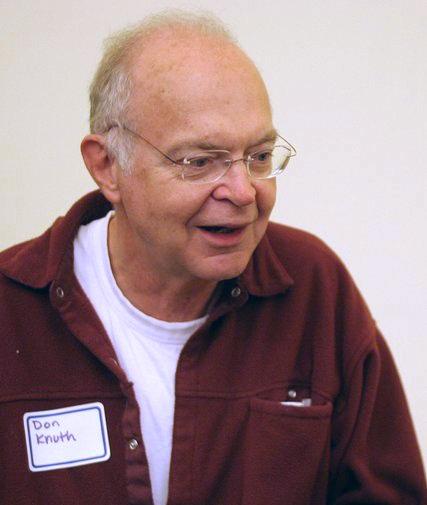
\includegraphics[width=\textwidth]{img/KnuthAtOpenContentAlliance}\\[6pt]
      \small\href{http://commons.wikimedia.org/wiki/File:KnuthAtOpenContentAlliance.jpg}{wikimedia commons}
    \end{figure}
  \end{column}
  \begin{column}{.6\textwidth}
    \large
    Programmers waste enormous amounts of time thinking about, or worrying about, the speed of noncritical parts of their programs, and these attempts at efficiency actually have a strong negative impact when debugging and maintenance are considered. We should forget about small efficiencies, say about $\unit[97]{\%}$ of the time: \textbf{premature optimization is the root of all evil}. \only<2->{Yet we should not pass up our opportunities in that critical $\unit[3]{\%}$.}\\[12pt]
    \begin{raggedright}
      \small{Donald E. Knuth, \cite{Knuth74structuredprogramming}}
    \end{raggedright}
  \end{column}
\end{columns}
\end{frame}

\begin{frame}
\frametitle{\insertsection{}}
\begin{center}
  \huge\textcolor{red}{Warning!}
\end{center}
\begin{columns}[c]
  \begin{column}{.35\textwidth}
    \begin{figure}[htb]
      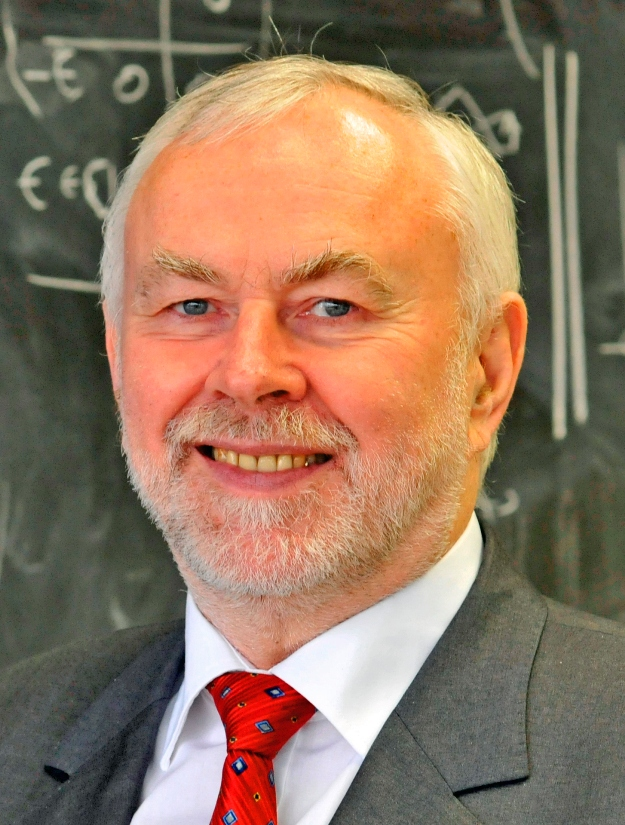
\includegraphics[width=\textwidth]{img/MartinGroetschel}\\[6pt]
      \small\href{http://www.zib.de/groetschel/Meine-Galerie/MartinGroetschel.JPG.html}{homepage of Martin Gr\"otschel}
    \end{figure}
  \end{column}
  \begin{column}{.6\textwidth}
\large
  \dots observes that a benchmark production planning model solved using linear programming would have taken 82 years to solve in 1988, using the computers and the linear programming algorithms of the day. Fifteen years later - in 2003 - this same model could be solved in roughly 1 minute, an improvement by a factor of roughly 43 million. Of this, a factor of roughly 1,000 was due to increased processor speed, \alert<2->{whereas a factor of roughly 43,000 was due to improvements in algorithms}!\\[12pt]
  \begin{raggedright}
    \small{Martin Gr\"otschel, cited in \cite{DesigningDigitalFuture}}
  \end{raggedright}
  \end{column}
\end{columns}
\end{frame}


\begin{frame}
\frametitle{\insertsection{}}
\begin{center}
  \huge\textcolor{red}{If and only if you have the feeling that your }
\end{center}
\begin{figure}[htb]
\includegraphics[height=0.5\textheight]{tikz/apod}\\[6pt]
Adapted from the APOD Cycle \cite{CUDABestPractises}
\end{figure}
\end{frame}

\part{Performance}
%\section[Performance]{Performance}
\section{A Definition}
\begin{frame}
\frametitle{\insertsectionhead{} : \insertpart{}
}
\vfill
\begin{block}{Etymology}
  \begin{description}
  \item[perform] from Middle English \textit{performen}, \textit{parfournen} (``to perform''), from Anglo-Norman \textit{performer}, \textit{parfourmer}, alteration of Old French \textit{parfornir}, \textit{parfurnir} (``to complete, accomplish, perform''), from \textit{par}- + \textit{fornir}, \textit{furnir} (``to accomplish, furnish''), \dots
  \item[ance] added to the stem of a verb to form a noun indicating a state or condition, such as result or capacity, associated with the verb.\\
    \begin{flushright}
      \small(\href{http://en.wiktionary.org/wiki/perform}{wiktionary})
    \end{flushright}
  \end{description}
\end{block}
\vfill
\begin{block}{Computer Performance}
  \begin{center}
    \dots is characterized by the amount of \alert<2->{useful work} accomplished by a computer system or computer network compared to the \alert<3->{time} and \alert<4->{resources} used.\\
  \end{center}
  \begin{flushright}
    \small(\href{http://en.wikipedia.org/wiki/Computer_performance}{wikipedia})
  \end{flushright}

  \end{block}
\vfill
\end{frame}

\section[Resources]{The resources used}
\subsection{Computers?}
\begin{frame}[c]
\frametitle{\insertsectionhead{}: \insertsubsection{}}
\begin{figure}[htb]
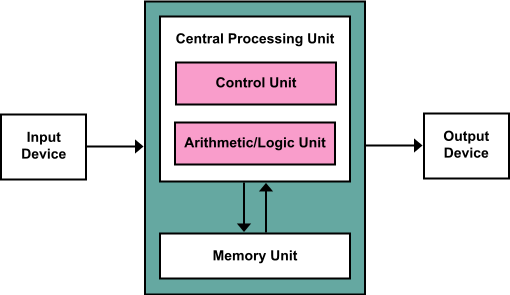
\includegraphics[height=0.65\textheight]{img/Von_Neumann_Architecture}\\[12pt]\Large
Stored-Program Computer Architecture (\cite{VonNeumann}, source: \href{http://en.wikipedia.org/wiki/Von_Neumann_architecture}{wikipedia})
\end{figure}
\end{frame}

\subsection{From Source To Instruction}
\begin{frame}[fragile]
\frametitle{\insertsectionhead{}: \insertsubsection{}}
\begin{block}{A simple app}
  \small
  \begin{pyglist}[language=c++,numbers=left,style=emacs]
  #include <iostream>

  int main(int argc, char *argv[])
  {
    int i = 42;
    std::cout << "i = " << i << "\n";
    return 0;
  }
  \end{pyglist}
\end{block}
\pause
\begin{block}{\texttt{g++ simple\_app.cpp -o simple\_app}}
  \small
  \begin{pyglist}[language=cpp-objdump,numbers=left,style=emacs]
    00000000004007e0 <main>:
    % ...
    4007ef:	c7 45 fc 2a 00 00 00 	movl   $0x2a,-0x4(%rbp)
    4007f6:	be 10 09 40 00       	mov    $0x400910,%esi
    4007fb:	bf 60 10 60 00       	mov    $0x601060,%edi
    400800:	e8 db fe ff ff       	callq  4006e0 <_ZStlsISt11char_traitsIcEERSt13basic_ostreamIcT_ES5_PKc@plt>
    % ...
    400825:	c3                   	retq
  \end{pyglist}
  % $
    
\end{block}
\end{frame}

\begin{frame}
\frametitle{\insertsectionhead{}: \insertsubsection{}}
\begin{figure}[htb]
\includegraphics<1>[height=0.65\textheight]{tikz/cachebased_microprocessor_matrix_memory_as_qm}
\includegraphics<2->[height=0.65\textheight]{tikz/cachebased_microprocessor_matrix}
\\[12pt]\large
Block diagram Cache-based microprocessor (adapted from \cite{HagerWelleinIntroHPC}, Fig. 1.2)
\end{figure}
\end{frame}


\subsection{From Disk to Memory}
\begin{frame}
\frametitle{\insertsectionhead{}: \insertsubsection{}}
  
\begin{columns}[c]
  \begin{column}{.45\textwidth}
    \begin{figure}[htb]
      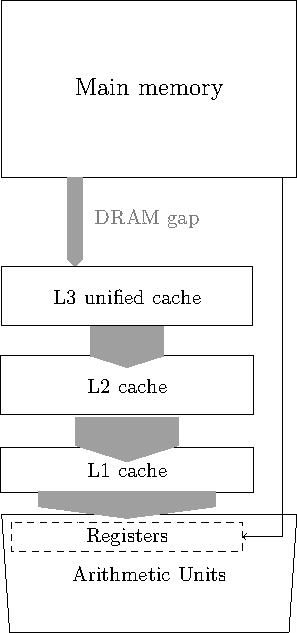
\includegraphics[height=0.78\textheight]{tikz/dram_gap}\\[2pt]\footnotesize
      (adapted from \cite{HagerWelleinIntroHPC}, Fig. 1.3)
    \end{figure}
  \end{column}
  \begin{column}{.45\textwidth}
    \vfill
    \begin{block}{Memory hierarchy of a cache-based microprocessor}
      \begin{itemize}
      \item direct access to RAM offers lowest bandwidth (slow)
      \item transfer bandwidth increases the closer the CPU is
      \item caches hide low RAM bandwidth by buffering hot data
      \item smallest transfer datum between caches:
        \textbf{cache line} $= \unit[64]{B}$
      \end{itemize}
    \end{block}
    \vfill
    % laptop CPU, Intel(R) Core(TM) i7-3520M CPU @ 2.90GHz (Ivy Bridge)
    % $ getconf -a /usr|grep -i CACHE
    % LEVEL1_ICACHE_SIZE                 32768
    % LEVEL1_ICACHE_ASSOC                8
    % LEVEL1_ICACHE_LINESIZE             64
    % LEVEL1_DCACHE_SIZE                 32768
    % LEVEL1_DCACHE_ASSOC                8
    % LEVEL1_DCACHE_LINESIZE             64
    % LEVEL2_CACHE_SIZE                  262144
    % LEVEL2_CACHE_ASSOC                 8
    % LEVEL2_CACHE_LINESIZE              64
    % LEVEL3_CACHE_SIZE                  4194304
    % LEVEL3_CACHE_ASSOC                 16
    % LEVEL3_CACHE_LINESIZE              64
    % server grade CPU, Intel(R) Xeon(R) CPU E5-2630 0 @ 2.30GHz (Sandy Bridge)
    % $ getconf -a /usr|grep -i CACHE
    % LEVEL1_ICACHE_SIZE                 32768
    % LEVEL1_ICACHE_ASSOC                8
    % LEVEL1_ICACHE_LINESIZE             64
    % LEVEL1_DCACHE_SIZE                 32768
    % LEVEL1_DCACHE_ASSOC                8
    % LEVEL1_DCACHE_LINESIZE             64
    % LEVEL2_CACHE_SIZE                  262144
    % LEVEL2_CACHE_ASSOC                 8
    % LEVEL2_CACHE_LINESIZE              64
    % LEVEL3_CACHE_SIZE                  15728640
    % LEVEL3_CACHE_ASSOC                 20
    % LEVEL3_CACHE_LINESIZE              64
    % server grade CPU, Intel(R) Xeon(R) CPU E5-2640 0 @ 2.50GHz (Sandy Bridge)
    % $ getconf -a /usr|grep -i CACHE
    % LEVEL1_ICACHE_SIZE                 32768
    % LEVEL1_ICACHE_ASSOC                8
    % LEVEL1_ICACHE_LINESIZE             64
    % LEVEL1_DCACHE_SIZE                 32768
    % LEVEL1_DCACHE_ASSOC                8
    % LEVEL1_DCACHE_LINESIZE             64
    % LEVEL2_CACHE_SIZE                  262144
    % LEVEL2_CACHE_ASSOC                 8
    % LEVEL2_CACHE_LINESIZE              64
    % LEVEL3_CACHE_SIZE                  15728640
    % LEVEL3_CACHE_ASSOC                 20
    % LEVEL3_CACHE_LINESIZE              64
    % server grade CPU, Intel(R) Xeon(R) CPU E3-1245 v3 @ 3.40GHz
    % $ getconf -a /usr|grep -i CACHE
    % LEVEL1_ICACHE_SIZE                 32768
    % LEVEL1_ICACHE_ASSOC                8
    % LEVEL1_ICACHE_LINESIZE             64
    % LEVEL1_DCACHE_SIZE                 32768
    % LEVEL1_DCACHE_ASSOC                8
    % LEVEL1_DCACHE_LINESIZE             64
    % LEVEL2_CACHE_SIZE                  262144
    % LEVEL2_CACHE_ASSOC                 8
    % LEVEL2_CACHE_LINESIZE              64
    % LEVEL3_CACHE_SIZE                  8388608
    % LEVEL3_CACHE_ASSOC                 16
    % LEVEL3_CACHE_LINESIZE              64
    \begin{block}{Common Dimensions}
      \begin{tabular}[h]{lr}
        L3 unified cache & $\unit[4-15]{MB}$ \\
        L2 cache & $N_{c}\times\unit[256]{KB}$ \\
        L1 cache & $N_{c}\times2\times\unit[32]{KB}$
      \end{tabular}
    \end{block}
    \vfill
  \end{column}
\end{columns}
\end{frame}

\begin{frame}
\frametitle{\insertsectionhead{}: \insertsubsection{}}
\begin{figure}[htb]
      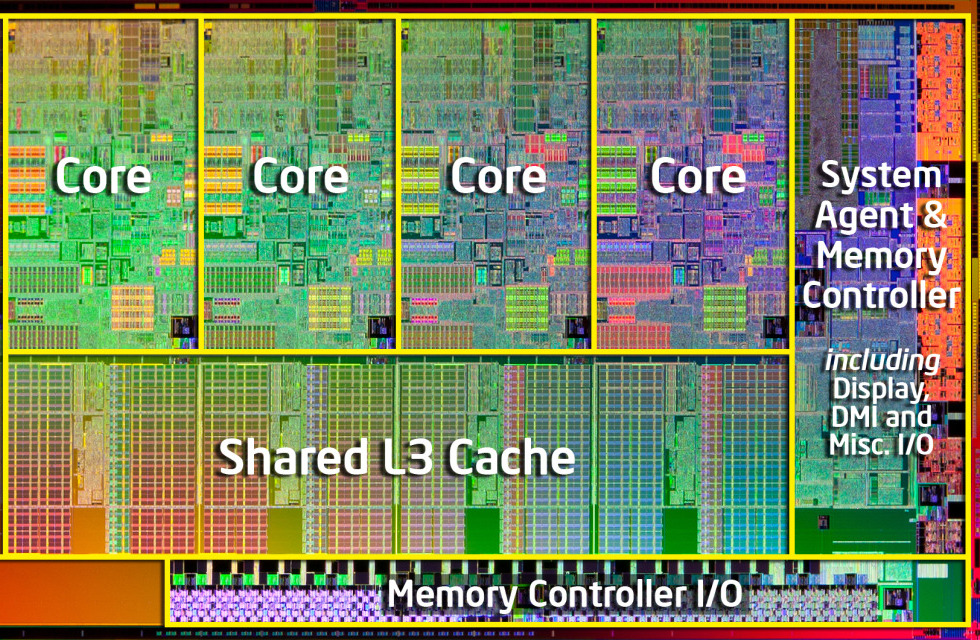
\includegraphics[height=0.65\textheight]{img/sandy-bridge-die-map_noIGP}\\[2pt]\small
      Intel\textregistered{} Sandy Bridge \textregistered{} die map (from \href{http://www.bit-tech.net/hardware/cpus/2011/01/03/intel-sandy-bridge-review/1}{bit-tech.net})
    \end{figure}
    \begin{center}\large
      \alert{Memory related parts of die make up $>\unit[50]{\%}$ of
        die area!}
    \end{center}
\end{frame}


\subsection{Wrapping up}
\begin{frame}
\frametitle{\insertsectionhead{}: \insertsubsection{}}
\begin{figure}[htb]
  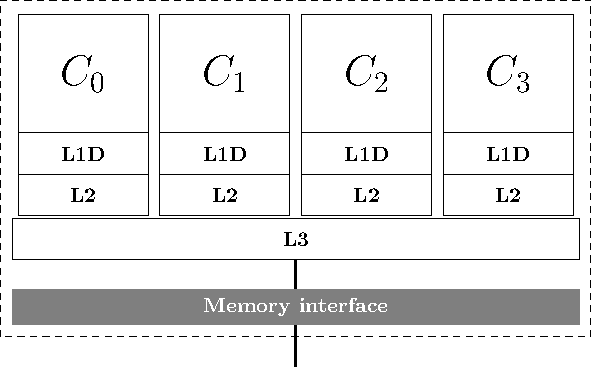
\includegraphics[height=0.55\textheight]{tikz/cpu_schematic}
\end{figure}
\begin{block}{CPUs are complicated beasts}
  \begin{columns}[t]
    \begin{column}{.48\textwidth}
      \begin{itemize}
      \item pipelined functional units
      \item superscaler arithmetic units
      \item out-of-order execution
      \end{itemize}
    \end{column}
    \begin{column}{.48\textwidth}
      \begin{itemize}
      \item symmetric multi-threading
      \item turbo-boost
      \item \dots
      \end{itemize}
    \end{column}
  \end{columns}
\end{block}

\end{frame}

\subsection{Exploring it}
\begin{frame}[fragile]
\frametitle{\insertsectionhead{}: \insertsubsection{}}
\begin{block}{stream benchmark \cite{McCalpin1995,McCalpin2007}}
  \begin{itemize}
  \item (one) standard candle of HPC benchmark(s)
  \item contains 4 functions that run on synthetic arrays 
  \item get it at: \href{http://www.cs.virginia.edu/stream/}{cs.virginia.edu/stream/}
  \end{itemize}
\end{block}
\begin{columns}
  \begin{column}{.17\textwidth}
    \hfill
  \end{column}
  \begin{column}{.6\textwidth}
    \begin{pyglist}[language=c++,numbers=left,style=emacs]
      float a[MAX], b[MAX], c[MAX];
  
      for(long i = 0;i<MAX;++i) { 
        a[i] = b[i]; //Copy 
        a[i] = d*b[i]; //Scale 
        a[i] = b[i]+c[i]; //Add 
        a[i] = b[i]+d*c[i]; //Triad }
    \end{pyglist}
  \end{column}
  \begin{column}{.17\textwidth}
    \hfill
  \end{column}
\end{columns}
\end{frame}

\begin{frame}
\frametitle{\insertsectionhead{}: \insertsubsection{}}
\huge
\begin{center}
  stream sweep
\end{center}
\end{frame}

\subsection{Summary}
\begin{frame}
\frametitle{\insertsectionhead{}: \insertsubsection{}}
\begin{columns}[c]
  \begin{column}{.35\textwidth}
    \begin{center}
      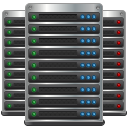
\includegraphics[height=0.3\textheight]{img/iconfinder_data-center}
    \end{center}
  \end{column}
  \begin{column}{.2\textwidth}
    \begin{center}
      
\includegraphics[height=0.2\textheight]{img/openclipart_not_equal} 
    \end{center}
  \end{column}
  \begin{column}{.35\textwidth}
    \begin{center}
      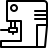
\includegraphics[height=0.3\textheight]{img/iconfinder_coffee_machine}
    \end{center}
  \end{column}
\end{columns}
\begin{center}
  \small (source: \href{www.iconfinder.com}{iconfinder.com},
  \href{openclipart.org}{openclipart.org})
\end{center}
\begin{itemize}\large
\item<1-> today's hardware composed of very advanced microprocessors (many years of engineering, moore's law, physics and material's science)
\item<2-> depending on the goal of your software development practise, intimate knowledge of the hardware is vital, beneficial or an extra
\item<3-> to understand performance bottlenecks, knowing the hardware concepts is crucial 
\end{itemize}

\end{frame}

\section{Profiling}
\begin{frame}
\frametitle{\insertsectionhead{}}
\begin{columns}[c]
  \begin{column}{.4\textwidth}
    \begin{center}
      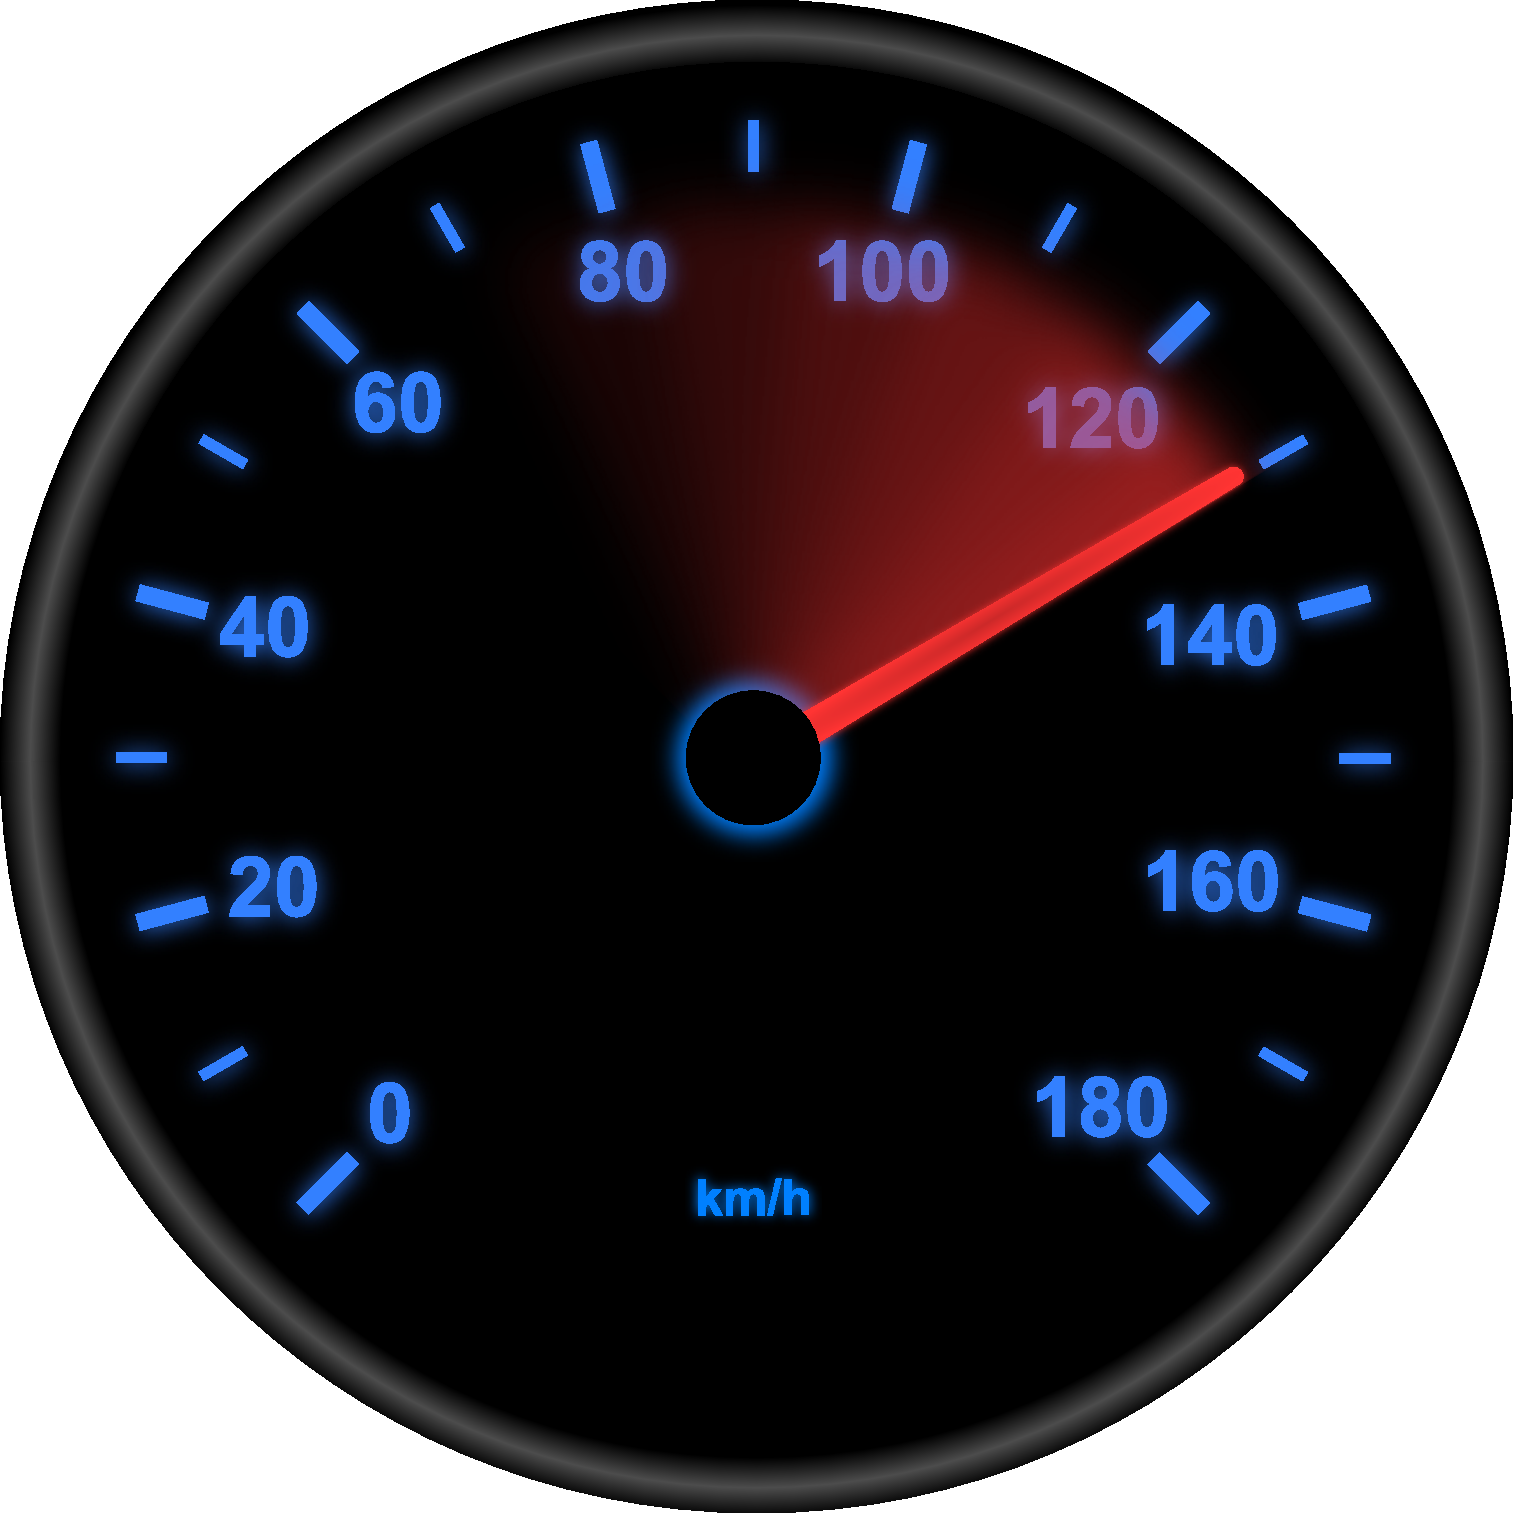
\includegraphics[width=.8\textwidth]{img/kmh_speedometer}
    \end{center}
    \end{column}
    \begin{column}{.55\textwidth}
      In software engineering, \textbf{profiling} \dots is a form of dynamic program analysis that \alert{measures}, for example, the space (memory) or time complexity of a program, the usage of particular instructions, or frequency and duration of function calls. \textit{The most common use of profiling information is to aid program optimization.}
      \begin{flushright}
        \small(\href{http://en.wikipedia.org/wiki/Profiling_(computer_programming)}{wikipedia})
      \end{flushright}
    \end{column}
  \end{columns}
\end{frame}

\subsection{\texttt{time} et al}
\begin{frame}[fragile]
\frametitle{\insertsectionhead{}: \insertsubsectionhead{}}
\vfill
\begin{block}{time}
  \begin{columns}[t]
    \begin{column}{.48\textwidth}
  \begin{pyglist}[language=bash,style=emacs]
  $ time sleep 10 #bash built-in
  
  real    0m10.001s
  user    0m0.000s
  sys     0m0.000s
\end{pyglist}  
    \end{column}
    \begin{column}{.48\textwidth}
 \begin{pyglist}[language=bash,style=emacs]
  $ `which time` -p sleep 10 #app

  real 10.00
  user 0.00
  sys 0.00
\end{pyglist}  
    \end{column}
  \end{columns}
\end{block}
\vfill
\begin{itemize}
\item simple and effective
\item use the ``user'' time (or the wallclock time) as central measurement unit
\item CPU time is an accumulated time (does not account for waits/sleeps)
\item does apply for library based timers (\texttt{boost::cpu\_time}, \texttt{std::chrono}, \dots)
\end{itemize}
\vfill
\end{frame}

\subsection{\texttt{valgrind}}
\begin{frame}
\frametitle{\insertsectionhead{}: \insertsubsectionhead{}}
  \begin{columns}[t]
    \begin{column}{.58\textwidth}
      \begin{itemize}
      \item originally memory profiling/debugging tool
      \item now: tool suite and framework for dynamic program analysis
      \item open-source tool under GPL
      \item runs ``instrumented'' application inside a VM
      \item apps take $>2-10\times$ longer inside \texttt{valgrind}
      \item applications should contain debugging symbols
      \end{itemize}
    \end{column}
    \begin{column}{.4\textwidth}
      \begin{center}
      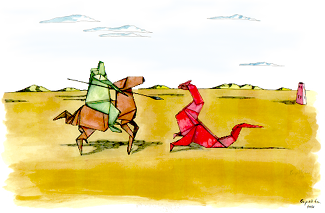
\includegraphics[width=\textwidth]{img/Valgrind_logo}
    \end{center}
    \end{column}
  \end{columns}
  \pause
  \begin{block}{parts concerning profiling}
    \begin{description}
    \item[memcheck] unallowed memory access, use of uninitialised values, memory leaks, bad \texttt{free}/\texttt{delete} calls
    \item[callgrind]  simulates L1i/d and L2 caches, records callgraph and logs memory access and instruction calls by line of source code (use \href{http://kcachegrind.sourceforge.net/html/Home.html}{kcachegrind} for visiualisation)
    \item[massif] heap profiling by taking regular snapshots of a program's heap (use \href{https://gitorious.org/massif-visualizer}{massif-visualizer}
    \end{description}
    \pause
    \begin{center}
      \alert{Let's take a tour!} (stream, ellbow-out)
    \end{center}
  \end{block}
\end{frame}


\subsection{\texttt{perf}}
\begin{frame}
\frametitle{\insertsectionhead{}: \insertsubsectionhead{}}
\begin{columns}[t]
    \begin{column}{.65\textwidth}
      \begin{itemize}
      \item performance analysis tool integrated into Linux kernel (since $2.6.31$)
      \item samples software/hardware performance counters at fixed rate
      \item open-source tool under GPL
      \item per application or system-wide profiling possible
      \item more details: \href{https://perf.wiki.kernel.org/index.php/Main_Page}{perf wiki}
      \end{itemize}
    \end{column}
    \begin{column}{.3\textwidth}
      \begin{center}
      
\includegraphics[width=\textwidth]{img/Tux}
    \end{center}
    \end{column}
  \end{columns}
  \pause
  \begin{block}{subcommands}
    \begin{description}
    \item[perf stats] receive quick performance summary of an application
    \item[perf record] record performance profile of an application (\texttt{perf.data} is created)
    \item[perf report] browse performance profile  
      \end{description}
    \pause
    \begin{center}
      \alert{Let's take a tour!} (again: stream, ellbow-out)
    \end{center}
  \end{block}

\end{frame}


\part{Tour de Force}
\section{The Burdens of Design}
\subsection{Inheritance}

\begin{frame}[fragile]
\frametitle{\insertsectionhead{}: \insertsubsectionhead{}}
 \begin{pyglist}[language=c++,numbers=left,style=emacs]
   struct Direct
   {
     int Perform(int &ia) { return --ia; }
   };

   struct AbstrBase
   {
     virtual int Perform(int &ia)=0;
   };

   struct Derived: public AbstrBase
   {
     virtual int Perform(int &ia) { return --ia; }
   };
   
   int main(int argc, char* argv[]){
     //...
     int begin = 1 << 30;
     while( direct_ptr->Perform(ia) );
     //...
   }
 \end{pyglist}
\end{frame}

\begin{frame}
\frametitle{\insertsectionhead{}: \insertsubsectionhead{}}
\begin{block}{g++ $4.8.2$}
  \begin{semiverbatim}
    Direct          2.66 ms from 1073741824 iterations
    Virtual         12.355 ms from 1073741824 iterations
  \end{semiverbatim}
\end{block}
\pause
\begin{block}{g++ $4.8.2$, \texttt{-O2}}
  \begin{semiverbatim}
    Direct  	    0 ms from 1073741824 iterations 
    Virtual 	7.317 ms from 1073741824 iterations
  \end{semiverbatim}
\end{block}
\end{frame}


\begin{frame}
\frametitle{\insertsectionhead{}: \insertsubsectionhead{}}
\begin{block}{Virtual Table (\texttt{vtable})}
  \begin{semiverbatim}
*** Dumping AST Record Layout
   0 | class Derived
   0 |   class AbstrBase (primary base)
   0 |     (AbstrBase vtable pointer)
   0 |     (AbstrBase vftable pointer)
     | [sizeof=8, dsize=8, align=8
     |  nvsize=8, nvalign=8]
  \end{semiverbatim}
\end{block}

\begin{itemize}
\item \texttt{vtable} $=$ binary tree of function pointers
\item evaluated at \textbf{runtime}
\item adds $\unit[64]{bit}$ pointer to class memory footprint
\item adds arbitrary amounts of pointer indirections to program flow
\end{itemize}

\end{frame}

\subsection{Over-Objectivism}
\begin{frame}
\frametitle{\insertsectionhead{}: \insertsubsectionhead{}}
\begin{columns}[c]
    \begin{column}{.45\textwidth}
      \begin{block}{$l_2$ norm of 3D image stacks}
        \begin{itemize}
        \item image stacks made from $n_x \times n_y \times n_z$ pixels
        \item typically obtained in microscopy, NMR, CT, \dots
        \item compare two stacks $f(x,y,z),g(x,y,z)$ of $N$ pixels by $l_2$-norm:\\
          $$ l_2 = \sum_{i \in N} (f_i - g_i)^2 $$
        \end{itemize}
      \end{block}
    \end{column}
    \begin{column}{.45\textwidth}
      \begin{center}
      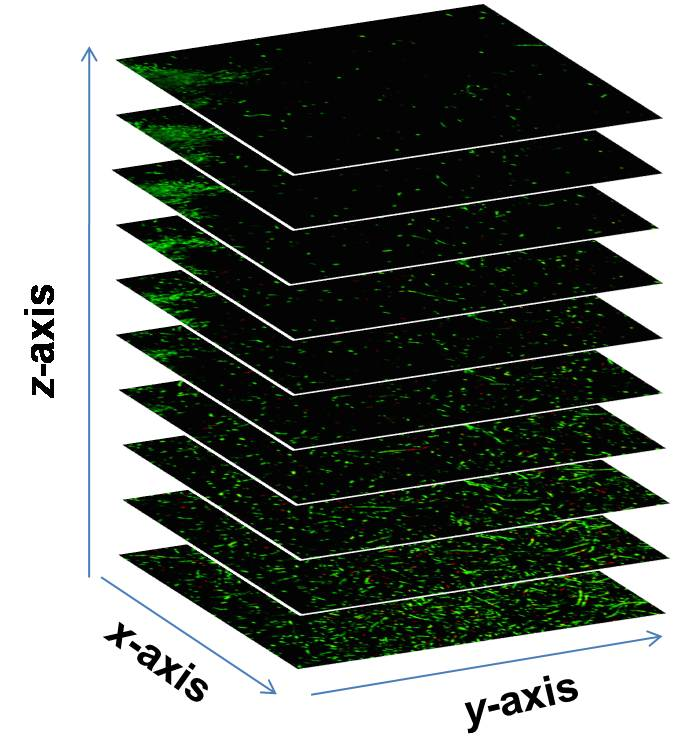
\includegraphics[width=\textwidth]{img/image_stack}\\[6pt]
      \small\href{http://bioimagel.com/3-d_operations}{placeholder}
    \end{center}
    \end{column}
  \end{columns}
\end{frame}

\begin{frame}[fragile]
\frametitle{\insertsectionhead{}: \insertsubsectionhead{}}
% \begin{columns}[t]
%     \begin{column}{.45\textwidth}
%       \begin{center}
%         \textbf{Array of Structures}
%       \end{center}
       \begin{pyglist}[language=c++,numbers=left,style=emacs]
         struct pixel {
          
          int x_;
          int y_;
          int z_;
          
          float intensity_;
          
        };
        
        struct pixel_stack {
          //...
          std::vector<pixel> data_;
          //...
        };
      \end{pyglist}
    % \end{column}
    % \begin{column}{.45\textwidth}
    %   \begin{center}
    %     \textbf{Structure of Arrays}
    %   \end{center}
      % \begin{pyglist}[language=c++,numbers=left,style=emacs]
        
      %   struct flat_stack   {
      %     //...
      %     std::vector<float> data_;
      %     std::vector<int> x_;
      %     std::vector<int> y_;
      %     std::vector<int> z_;
      %     //...
      %   };
      %   \end{pyglist}
        
  %   \end{column}
  % \end{columns}
 \end{frame}

% \begin{frame}
% \frametitle{\insertsectionhead{}: \insertsubsectionhead{}}
% \begin{center}
%   \huge timings for single core
% \end{center}
% \begin{itemize}
% \item prime example of ``nice'' design on small scales, performance problem on large scales
% \item segmentation of \texttt{pixel_stack} causes non-optimal use of caches
% \item prominent issue with hardware accelerators (they work extremely well with structure of arrays)
% \end{itemize}
% \end{frame}

% \subsection{Take-Home}
% \begin{frame}
% \frametitle{\insertsectionhead{}: \insertsubsectionhead{}}


% \end{frame}

\section{The Free Lunch}

\section{Vectorisation}


\part{Exercises}
\section{Tasks}
\section{Results}

\section{Literature}
\begin{frame}[c]
\frametitle{\insertsection{}}
\nocite{*}
\tiny%footnotesize
\bibliographystyle{ieeetr}
\bibliography{slides}
\end{frame}

\end{document}




